% Synthetic fixture: an invented diagram whose node text is set by lualatex
% in the repository's shipped faces (CID-keyed CFF in the PDF).
\documentclass{standalone}
\usepackage{tikz}
\usepackage{fontspec}
\usepackage{unicode-math}
\setmainfont{SourceSerifPro-Regular.otf}[Path=./fonts/, BoldFont=SourceSerifPro-Bold.otf]
\setmathfont{FiraMath-Regular.otf}[Path=./fonts/]
\begin{document}
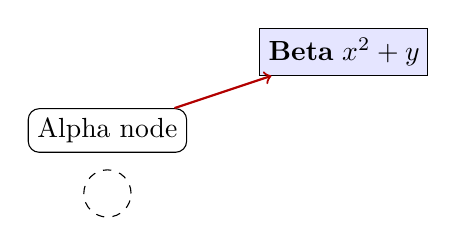
\begin{tikzpicture}
  \node[draw, rounded corners] (a) at (0,0) {Alpha node};
  \node[draw, fill=blue!10] (b) at (3,1) {\textbf{Beta} $x^2+y$};
  \draw[->, thick, red!70!black] (a) -- (b);
  \draw[dashed] (0,-0.8) circle (0.3);
\end{tikzpicture}
\end{document}
